%! Author = danielmendes
%! Date = 21.10.24
\chapter{Überblick}

\section{Einführung in Benchmarks}

Benchmarks dienen dazu, praktisch und effektiv zu untersuchen, wie sich ein
System unter Last verhält. Die wichtigste Erkenntnis, die man aus Benchmarks
gewinnen kann, sind die Probleme und Fehler, die man systematisch dokumentieren
und nach Priorität abarbeiten sollte. Das Ziel von Benchmarks ist die Reduzierung
und Bewertung von unerwünschtem Verhalten sowie die Analyse, wie sich das
System derzeit und unter simulierten, zukünftigen, anspruchsvolleren Bedingungen
verhalten könnte.

Es gibt zwei verschiedene Techniken für Benchmarks. Die erste zielt darauf ab,
die Applikation als Ganzes zu testen (full-stack). Dabei wird nicht nur die
Datenbank getestet, sondern die gesamte Applikation, einschließlich des Webservers,
des Netzwerks und des Applikationscodes. Der Ansatz dahinter ist, dass ein Nutzer
genauso lange auf eine Abfrage warten muss, wie das gesamte System benötigt.
Daher sollte diese Wartezeit so gering wie möglich sein. Es kann dabei vorkommen,
dass MySQL nicht immer das Bottleneck ist.\footnote{Gemeint ist ein Engpass beim Transport von Daten oder Waren, der maßgeblichen Einfluss auf die Abarbeitungsgeschwindigkeit hat. Optimierungsversuche an anderer Stelle führen oft nur zu geringen oder gar keinen messbaren Verbesserungen der Gesamtsituation. (\cite{bottleneck})}

Full-Stack-Benchmarks haben jedoch auch Nachteile. Sie sind schwieriger zu erstellen
und insbesondere schwieriger korrekt einzurichten. Wenn man lediglich verschiedene
Schemas und Abfragen in MySQL auf ihre Performance testen möchte, gibt es sogenannte
Single-Component-Benchmarks. Diese analysieren ein spezifisches Problem in der
Applikation und sind deutlich einfacher zu erstellen. Ein weiterer Vorteil besteht
darin, dass nur ein Teil des gesamten Systems getestet wird, wodurch die Antwortzeiten
kürzer sind und man schneller Ergebnisse erhält.

Wenn bei Benchmarks schlechte Designentscheidungen getroffen werden, kann dies zu einer
falschen Interpretation des Systems führen, da die Ergebnisse nicht die Realität widerspiegeln.
Die Größe des Datensatzes und des Workloads muss realistisch sein. Idealerweise verwendet
man einen Snapshot\footnote{Snapshots bestehen größtenteils aus Metadaten, die den Zustand Ihrer Daten definieren, und sind keine vollständige Duplikation der Daten auf Ihrer Festplatte. Snapshots werden häufig für Test-/Entwicklungsaufgaben verwendet. (\cite{snapshot}) } des tatsächlichen produktiven Datensatzes.
Gibt es keine Produktionsdaten, sollten die Daten und der Workload simuliert werden,
da realistische Benchmarks komplex und zeitaufwendig sein können.

Häufige Fehler beim Durchführen von Benchmarks sind unter anderem, dass nur ein kleiner Teil
der tatsächlichen Datensatzgröße verwendet wird und die Datensätze unkorrekt gleichmäßig
verteilt sind. In der Realität können Hotspots auftreten. Bei zufällig generierten Werten
kommt es hingegen häufig zu unrealistisch gleichmäßig verteilten Datensätzen. Ein weiterer
Fehler besteht darin, dass man beim Testen einer Anwendung nicht das tatsächliche
Benutzerverhalten nachstellt. Wenn gleiche Abfragen in einer Schleife ausgeführt werden,
muss man außerdem auf das Caching achten, da sonst falsche Annahmen über die Performance
getroffen werden können. Zudem wird oft die Warmmachphase des Systems vollständig ignoriert.
Kurze Benchmarks können schnell zu falschen Annahmen über die Performance des Systems führen.

Um verlässliche Ergebnisse zu erhalten, sollte ein Benchmark ausreichend lange laufen,
um den stabilen Zustand des Systems zu beobachten, insbesondere bei Servern mit großen
Datenmengen und viel Speicher. Dabei ist es wichtig, so viele Informationen wie möglich zu
erfassen und sicherzustellen, dass der Benchmark wiederholbar ist, da unzureichende oder
fehlerhafte Tests wertlos sind. Außerdem ist es wichtig, die Ergebnisse in einem Diagramm
darzustellen, da auftretende Phänomene sonst anhand einer tabellarischen Darstellung nicht
erkannt werden können.


\section{Measures}
\begin{itemize}[label={--}]
    \item \textbf{Durchsatz (Throughput):} Der Durchsatz ist die Anzahl an Transaktionen pro Zeiteinheit.
    Er ist standardisiert, und Datenbankanbieter versuchen, diesen zu optimieren.
    Meistens werden Transaktionen pro Sekunde (oder manchmal pro Minute) als Einheit verwendet.
    \item \textbf{Antwortzeiten (Latenz):} Die Antwortzeit misst die gesamte Zeit, die für eine Abfrage benötigt wird.
    Diese kann, abhängig von der Applikation, in Mikrosekunden (µs), Millisekunden (ms), Sekunden oder Minuten angegeben werden.
    Von dieser Zeit können aggregierte Antwortzeiten wie Durchschnitt, Maximum, Minimum und Perzentile abgeleitet werden.
    Das Maximum ist oft eine weniger sinnvolle Metrik, da es sich nicht gut wiederholen lässt.
    Daher nutzt man eher Perzentile bei den Antwortzeiten.
    Wenn beispielsweise das 95. Perzentil der Antwortzeit bei 5 ms liegt, bedeutet dies, dass mit einer Wahrscheinlichkeit von 95 \% die Abfrage in weniger als 5 ms abgeschlossen ist.
    \item \textbf{Nebenläufigkeit (Concurrency):} Die Nebenläufigkeit auf dem Webserver lässt sich nicht zwangsläufig auf den Datenbankserver übertragen.
    Eine genauere Messung der Gleichzeitigkeit auf dem Webserver besteht darin, zu bestimmen, wie viele gleichzeitige Anfragen zu einem bestimmten Zeitpunkt ausgeführt werden.
    Es kann auch geprüft werden, ob der Durchsatz sinkt oder die Antwortzeiten steigen, wenn die Gleichzeitigkeit zunimmt.
    Beispielsweise benötigt eine Website mit „50.000 Benutzern gleichzeitig“ vielleicht nur 10 oder 15 gleichzeitig laufende Abfragen.
    \item \textbf{Skalierbarkeit (Scalability):} Skalierbarkeit ist wichtig für Systeme, die ihre Performance unter unterschiedlich starken Workloads beibehalten müssen.
    Ein ideales System würde doppelt so viele Abfragen beantworten (Throughput), wenn doppelt so viele „Arbeiter“ versuchen, die Aufgaben zu erfüllen.
    Die meisten Systeme sind jedoch nicht linear skalierbar und zeigen Leistungseinbußen, wenn die Parameter variieren.
\end{itemize}


\section{Tools}\label{sec:tools}

\subsection{Einführung}\label{subsec:einfuhrung}

Als Haupttool, um Benchmarktests durchzuführen, habe ich mich für Sysbench \cite{sysbench_repo}
entschieden. Sysbench ist ein Open-Source-Tool, das ein skriptfähiges, multi-threaded Benchmark-Tool
ist, das auf LuaJIT basiert. Es wird auch hauptsächlich für Datenbankbenchmarks verwendet, kann
jedoch auch dazu eingesetzt werden, beliebig komplexe Arbeitslasten zu erstellen, die keinen
Datenbankserver erfordern. Dabei werden Tests auf verschiedenen Systemressourcen, wie CPU, S
peicher, I/O und Datenbanken wie MySQL \cite{sysbench_mysql} verwendet.

Im Zuge der Recherchearbeit habe ich mir auch andere Benchmarking-Tools betrachtet, wie z.B.
Benchbase \cite{DifallahPCC13} oder mybench \cite{mybench_repo}. Die größten Vorteile von
Sysbench habe ich in der Skriptfähigkeit und Flexibilität gesehen. D.h. dass ich benutzerdefinierte
Benchmarks schneller und unkompliziert erstellen kann. Außerdem hat sich Sysbench als de facto
Standard im Bereich der Datenbankbenchmarks etabliert \cite{mybench_comparison}. Dadurch stehen
eine breite Nutzerbasis und viele verfügbare Ressourcen zur Verfügung. Im Vergleich zu den
anderen Tools bietet allerdings Sysbench eine weniger präzise Steuerung der Ergebnisrate
und der Transaktionen. Außerdem haben Tools wie mybench die Möglichkeit, in Echtzeit umfassende
Visualisierungen darzustellen. Damit können Metriken live in einem Diagramm angezeigt werden
\cite{mybench_user_interface}. Dieses Feature ist sicherlich hilfreich, aber in meinem Fall habe
ich abgewogen und bin zu dem Entschluss gekommen, dass die einfachere Bedienung für mich der
ausschlaggebende Grund, neben dem Fakt, dass Sysbench der de facto Standard ist.

Trotzdem kann man nicht komplett auf Graphen verzichten, da beispielweise Entwicklungen
im Laufe einer Zeitmessung in einem Kurvenverlauf deutlich besser zu erkennen sind als in einer CSV-Datei.
Anhand der reinen Zahlen aus diesen Tabellen fallen diese wiederkehrende Trends unter anderem nicht direkt auf.
Die Kennzahlen, die mithilfe von Sysbench ermittelt werden, werden in einer CSV-Datei gespeichert.
Um diese tabellarische Form in eine Grafische umzuwandeln, gibt es unterschiedliche Tools, die widerum
eigene Vor- und Nachteile bieten.

Die erste mögliche Alternative stellt das Tool Gnuplot \cite{gnuplot} dar.
Mit diesem lassen sich CSV-Dateien sehr gut darstellen. Wenn man aber beispielweise nur bestimmte Spalten
aus der Tabelle anzeigen lassen will, dann kommt man schnell an seine Granzen.
Um besser Anpassungsfähig sein zu können, habe ich mich letztlich dazu entschieden ein eigenes Python-Script
zu schreiben, die mithilfe der Libraries pandas (//TODO (Daniel): find source) matplotlib.pyplot (//TODO (Daniel): find source)
die Graphen erstellt.

\subsection{Einführung in die Tools}\label{subsec:einfuhrung-in-die-tools}

Als allererstes muss der MySQL-Server (oder eine anderes relationales Datenbankverwaltungssystem, das von Sysbench
unterstützt wird) lokal auf dem Rechner gestartet sein. Wichtig ist dabei die User -und Passwortdaten zu merken, da
diese von den Sysbench - Benchmarks benötigt werden. Nachdem das RDBMS gestartet worden ist, muss zudem eine
Datenbank erstellt werden. Dies könnte unter anderem so aussehen:

\begin{lstlisting}[label={lst:create database}]
CREATE DATABASE sbtest;
\end{lstlisting}

Nachdem man die Datenbank erstellt hat, muss das Tool Sysbench zunächst installiert werden.
Als nächstes machen wir uns mit dem Tool und den verschiedenen Argumenten,
die beim Aufruf mitübergeben werden müssen oder können, vertraut.
Hier ist eine Auflistung mit den übergebenen Argumenten:

\begin{itemize}
    \item \texttt{--db-driver}: Gibt den Treiber für die Datenbank an, die Sysbench verwenden soll. In diesem Fall \texttt{mysql}, um MySQL-Datenbanken zu testen.
    \item \texttt{--mysql-host}: Der Hostname oder die IP-Adresse des MySQL-Servers. Standardmäßig wird \texttt{localhost} verwendet, wenn nichts angegeben wird.
    \item \texttt{--mysql-user}: Der Benutzername, mit dem Sysbench auf die MySQL-Datenbank zugreift.
    \item \texttt{--mysql-password}: Das Passwort für den MySQL-Benutzer. Falls der Benutzer kein Passwort hat oder der Zugriff über eine andere Authentifizierungsmethode erfolgt, kann dieses Argument weggelassen werden.
    \item \texttt{--mysql-db}: Der Name der MySQL-Datenbank, auf die zugegriffen wird. In diesem Beispiel \texttt{sbtest}.
    \item \texttt{--time}: Gibt die Laufzeit des Benchmarks in Sekunden an und muss immer mit angegeben werden.
    \item \texttt{--report-interval}: Gibt das Intervall in Sekunden an, in dem Zwischenergebnisse während des Tests ausgegeben werden.
    Sofern \texttt{--report-interval} nicht gesetzt wird, werden die Ergebnisse erst am Ende des Tests angezeigt.
    \item \texttt{--tables}: Die Anzahl der Tabellen, die für den Test erstellt werden sollen. Standardmäßig wird nur eine Tabelle erstellt.
    \item \texttt{--table-size}: Die Anzahl der Datensätze (Zeilen) pro Tabelle. Muss auch nicht zwingend angegebend werden.
\end{itemize}

Neben den sieben aufgelisteten Argumenten gibt es zwei weitere wichtige Optionen:
\begin{enumerate}
    \item Wie im Abschnitt~\ref{einfuhrung} erwähnt, kann ein Lua-Skript angegeben werden, um eigene
    Tabellen zu erstellen, Beispieldaten einzufügen und bestimmte Abfragen durchzuführen.
    Dazu muss am Ende der Sysbench-Befehlszeile lediglich der Pfad zur Lua-Datei hinzugefügt werden.
    Ein erklärendes Beispiel dazu folgt weiter unten in diesem Abschnitt.
    \item Die Methode, den Sysbench ausführen soll, muss ebenfalls spezifiziert werden.
    Auch dieser wird am Ende der Sysbench-Befehlszeile angehängt.
\end{enumerate}

Zunächst schauen wir ein kurzes Demo-Beispiel, denn es gibt die Möglichkeit die Datenbank
auf Performance zu testen, ohne selbst eigene SQL-Befehle zu schreiben. Dafür gibt es vordefinierte Testtypen von Sysbench.
Auf diese Weise kann man schnell die Korrektheit der Einrichtung des Tools überprüfen, bevor man Lua-Scripts
für die eigenen Bedürfnisse schreibt.

Man kann unter anderen zwischen diesen Testtypen wählen:
\begin{itemize}
    \item \textbf{oltp\_insert}: Prüft die Fähigkeit der Datenbank, Daten schnell und effizient einzufügen und
    simuliert eine Umgebung, in der viele Schreiboperationen ausgeführt werden.
    \item \textbf{oltp\_read\_only}: Fokussiert sich auf die Performance bei Leseoperationen und
    eignet sich, um die Leistung bei einer rein lesenden Arbeitslast zu testen.
    \item \textbf{oltp\_read\_write}: Simuliert eine realistische Arbeitslast, bei der sowohl Lese- als
    auch Schreiboperationen gleichzeitig durchgeführt werden.
\end{itemize}

Des Weiteren gibt es auch unterschiedliche Methoden, die mit den Testtypen kombiniert werden können.

\begin{itemize}
    \item \item \textbf{prepare}: Bereitet die Datenbank für den Test vor, u.a. das Einfügen von benötigten Datensätze.
    \item \textbf{run}: Ist die Ausführungsphase des Tests. Je nach Testtyp führt diese Methode die spezifizierten Operationen aus,
    wie etwa das Einfügen von Daten (oltp\_insert), das Abfragen von Daten (oltp\_read\_only) oder beides (oltp\_read\_only).
    Dabei wird die Performance der Datenbank unter der angegebenen Arbeitslast gemessen.
    \item \textbf{cleanup}: Diese Methode sorgt dafür, dass nach Abschluss des Tests alle Testdaten entfernt werden.
    Sie stellt die Datenbank in ihren ursprünglichen Zustand zurück und stellt sicher,
    dass keine Testdaten zurückbleiben, die eine mögliche produktive Umgebung beeinträchtigen könnten.
\end{itemize}

Für das Demo-Beispiel wählen wir den Testtypen \textbf{oltp\_read\_write} und allen Methoden aus.
Für die Methode run würde unsere Query so aussehen, wobei \texttt{YOUR\_USER} und \texttt{YOUR\_PASSWORD}
entsprechend ersetzt werden müssten:

\begin{lstlisting}[style=custom_daniel,label={lst:sysbenchrun}]
sysbench oltp_read_write \
  --db-driver=mysql \
  --mysql-user=YOUR_USER \
  --mysql-password=YOUR_PASSWORD \
  --mysql-db="sbtest" \
  --time=10 \
  --report-interval=1 \
  run
\end{lstlisting}

Wenn man nur diese Query ausführt, fällt er auf, dass die Query scheitert. Deshalb bietet es sich an ein Shell-Script
zu schreiben, indem zuerst \texttt{prepare} aufgerufen wird und als Nächstes erst \texttt{run}. Die Ergebnisse der Log-Datei
speichert man sich dann in einer Datei und aus dieser Datei erstellt man eine CSV-Datei, mit der man später die Graphen
erstellen lässt. Und als letzten Schritt ruft man die \texttt{cleanup}-Methode auf, damit bei erneuter Ausführung keine
Fehler entstehen, bzw. die Produktivumgebung nicht gestört wird, wenn diese sonst beeinflusst werden würde.

Dies ist das Shell-Script, dass zuständig ist für den kompletten Ablauf:
\lstinputlisting[
    language=bash,
    caption=Sysbench Script,
    label={lst:sysbench_monitor},
    style=custom_daniel,
]{Scripts/Demo/sysbench_monitor.sh}

\lstinputlisting[
    language=gnuplot,
    caption=Gnuplot Script,
    label={lst:plot_sysbench},
    style=custom_daniel,
]{Scripts/Demo/plot_sysbench.gp}

Das Python-Script, das zuständig ist für die Graphgenerierung muss als Argument zum einen
die CSV-Datei übermittelt bekommen und zum anderen kann es nur eine bestimmte Auswahl an
Messwerten übergeben, damit nur für diese die Graphen erzeugt werden.
Dies ist das zuständige Python-Script:

\lstinputlisting[
    language=python,
    caption=Pandas Graph Generator,
    label={lst:pandas_plot},
    style=custom_daniel,
]{Scripts/Join_Type/generateplot.py}

% missing: how the script and results exactly are fpr Join_Type and explain the measures underneath


\begin{figure}[!ht]
    \centering
    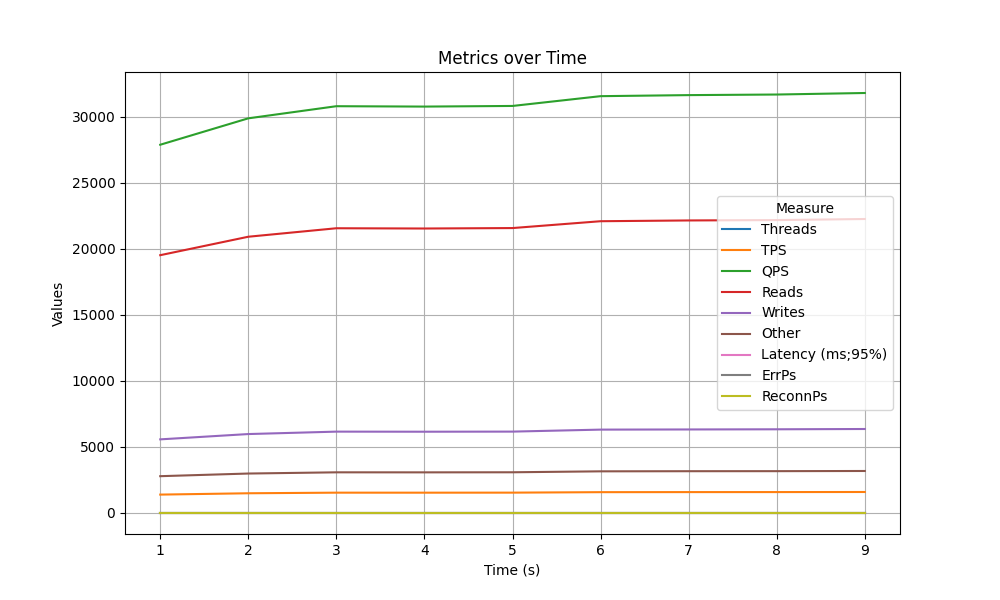
\includegraphics[width=.8\textwidth]{PNGs/Demo/Summary}
    \caption[Pandas - Beispiel]{Grafik generiert mithilfe des Pythontools Pandas}
    \label{demo-pandas}
\end{figure}

\begin{figure}[!ht]
    \centering
    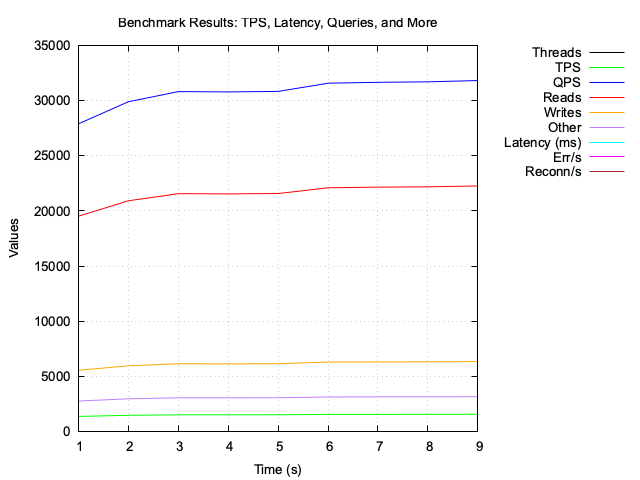
\includegraphics[width=.8\textwidth]{PNGs/Demo/sysbench_output}
    \caption[Gnuplot - Beispiel]{Grafik generiert mithilfe von Gnuplot}
    \label{demo-gnuplot}
\end{figure}


\begin{itemize}
    \item \textbf{Threads}: Die Anzahl der gleichzeitig verwendeten Threads.
    Mehr Threads können die Parallelität erhöhen, jedoch kann eine zu hohe Anzahl
    die Leistung beeinträchtigen, wenn das System überlastet wird.
    \item \textbf{TPS (Transactions Per Second)}: Die Anzahl der Transaktionen pro Sekunde.
    Ein höherer Wert deutet auf eine bessere Datenbankleistung hin.
    \item \textbf{QPS (Queries Per Second)}: Die Anzahl der Abfragen pro Sekunde.
    Ein höherer Wert ist besser und zeigt die Effizienz bei der Verarbeitung von Abfragen.
    \item \textbf{Reads}: Die Anzahl der Leseoperationen.
    Mehr Leseoperationen sind im Allgemeinen besser, da sie eine höhere Datenauslastung anzeigen, was jedoch auch vom spezifischen Anwendungsfall abhängt.
    \item \textbf{Writes}: Die Anzahl der Schreiboperationen.
    Ähnlich wie bei den Leseoperationen: Mehr Schreibvorgänge sind besser, solange die Performance erhalten bleibt.
    \item \textbf{Other}: Bezieht sich auf andere Arten von Operationen, die weder als Reads noch als Writes kategorisiert werden.
    Ein höherer Wert ist gut, solange er nicht zu einer Überlastung führt.
    \item \textbf{Latency (ms; 95\%)}: Die durchschnittliche Zeit in Millisekunden, die benötigt wird, um Anfragen zu bearbeiten, wobei der Wert im 95. Perzentil betrachtet wird.
    Niedrigere Werte sind besser, da sie auf schnellere Reaktionszeiten hinweisen.
    \item \textbf{ErrPs (Errors Per Second)}: Die Anzahl der Fehler pro Sekunde.
    Ein niedriger Wert ist wünschenswert, da er auf eine höhere Stabilität und Zuverlässigkeit des Systems hinweist.
    \item \textbf{ReconnPs (Reconnects Per Second)}: Die Anzahl der Wiederverbindungen pro Sekunde.
    Ein niedrigerer Wert ist ebenfalls besser, da häufige Wiederverbindungen auf Stabilitätsprobleme hindeuten können.
\end{itemize}
